\section{State-of-the-Art Classification Methods}

\subsection{Classification methods}
	In this project, the following classification methods are used to classify the data:

	\subsubsection{Support Vector Machine (SVM)}
	SVM is a supervised learning model with associated learning algorithms that analyze data used for classification and regression analysis. Given a set of training examples, each marked as belonging to one of two categories, an SVM training algorithm builds a model that assigns new examples to one category or the other, making it a non-probabilistic binary linear classifier.
	
	\subsubsection{Random Forest (RF)}
	Random forests or random decision forests are an ensemble learning method for classification, regression and other tasks, that operate by constructing a multitude of decision trees at training time and outputting the class that is the mode of the classes (classification) or mean prediction (regression) of the individual trees. It internally uses decision tree as a base classifier. 
	
	\subsubsection{K-Nearest Neighbors (k-NN)}
	In pattern recognition, the k-nearest neighbors algorithm (k-NN) is a non-parametric method used for classification and regression. In both cases, the input consists of the k closest training examples in the feature space. The output depends on whether k-NN is used for classification or regression. In k-NN classification, the output is a class membership. An object is classified by a majority vote of its neighbors, with the object being assigned to the class most common among its k nearest neighbors (k is a positive integer, typically small). If $k = 1$, then the object is simply assigned to the class of that single nearest neighbor.

	\subsubsection{Gaussian Naive Bayes (GNB)}
	In machine learning, naive Bayes classifiers are a family of simple probabilistic classifiers based on applying Bayes' theorem with strong (naive) independence assumptions between the features. They are among the simplest Bayesian network models. But they could be coupled with Kernel Density Estimation (KDE) to handle continuous data. Naive Bayes has been studied extensively since the 1950s. It was introduced under a different name into the text retrieval community in the early 1960s, and remains a popular (baseline) method for text categorization, the problem of judging documents as belonging to one category or the other (such as spam or legitimate, sports or politics, etc.) with word frequencies as the features. With appropriate pre-processing, it is competitive in this domain with more advanced methods including support vector machines. It also finds application in automatic medical diagnosis.
	
	\subsubsection{Decision Tree Classifier (DTC)}
	Decision tree learning uses a decision tree (as a predictive model) to go from observations about an item (represented in the branches) to conclusions about the item's target value (represented in the leaves). It is one of the predictive modelling approaches used in statistics, data mining and machine learning. Tree models where the target variable can take a discrete set of values are called classification trees; in these tree structures, leaves represent class labels and branches represent conjunctions of features that lead to those class labels. Decision trees where the target variable can take continuous values (typically real numbers) are called regression trees.
	
	\subsubsection{Linear Discriminant Analysis (LDA)}
	In statistics, linear discriminant analysis (LDA), normal discriminant analysis (NDA), or discriminant function analysis is a generalization of Fisher's linear discriminant, a method used in statistics, pattern recognition and machine learning to find a linear combination of features that characterizes or separates two or more classes of objects or events. The resulting combination may be used as a linear classifier, or, more commonly, for dimensionality reduction before later classification.


	\begin{table}
		\centering
		\begin{tabular}{|c|c|c|c|c|c|c|c|}
			\hline
				\textbf{Algorithm} &\textbf{Accuracy} &\textbf{Precision} &\textbf{Recall} &\textbf{F1} &\textbf{E.T. (Sec)} \\ \hline
				\hline
				DTC   & 0.442   & 0.449   & 0.442  & 0.436 & 0.004 \\ \hline
				GNB   & 0.206   & 0.182   & 0.206  & 0.183 & 0.003 \\ \hline
				KNN   & 0.358   & 0.379   & 0.358  & 0.352 & 0.008 \\ \hline
				LDA   & 0.245   & 0.206   & 0.245  & 0.203 & 0.003 \\ \hline
				RFC   & 0.473   & 0.482   & 0.473  & 0.468 & 0.182 \\ \hline
				SVM   & 0.282   & 0.253   & 0.282  & 0.219 & 0.168 \\ 
			\hline
		\end{tabular}
		\caption{Classifier performance before dimensionality reduction and hyperparameter optimization}
		\label{tab:performance_before}
	\end{table}




	\begin{figure}[H]
		\centering
		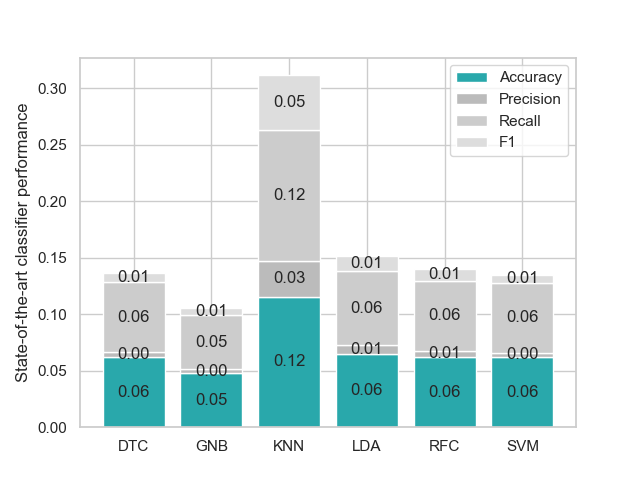
\includegraphics[width=0.5\textwidth]{Plots/Performance_before.png}
		\caption{Classifier performance before dimensionality reduction and hyperparameter optimization}
		\label{fig:performance_before}
	\end{figure}

\subsection{Evaluation methods}
	The evaluation methods used in this project are:
	\subsubsection{Cross-validation}
		Cross-validation is performed using the Stratified K-Fold technique to evaluate the performance of each classifier. Metrics such as \emph{accuracy}, \emph{precision}, \emph{recall} and \emph{F1-score} are calculated and recorded. The results are aggregated and displayed in tabular form, providing insights into the initial accuracy and performance of each classifier. The results are also visualized using a bar chart to provide a more intuitive comparison between the classifiers. 
	\subsubsection{Confusion matrix}
		Confusion matrices are generated to visualize the classification performance of each refined classifier. Heatmap of the correlation matrix for the original features are also created to show correlations among features. 

	The evaluation is performed before and after the feature selection and hyperparameter optimization process to determine the effect of feature selection and hyperparameter optimization on the performance of each classifier. 
	
